%  LaTeX support: latex@mdpi.com
%  For support, please attach all files needed for compiling as well as the log file, and specify your operating system, LaTeX version, and LaTeX editor.

%=================================================================
% pandoc conditionals added to preserve backwards compatibility with previous versions of rticles

\documentclass[notspecified,article,submit,moreauthors,pdftex]{Definitions/mdpi}


%% Some pieces required from the pandoc template
\setlist[itemize]{leftmargin=*,labelsep=5.8mm}
\setlist[enumerate]{leftmargin=*,labelsep=4.9mm}


%--------------------
% Class Options:
%--------------------

%---------
% article
%---------
% The default type of manuscript is "article", but can be replaced by:
% abstract, addendum, article, book, bookreview, briefreport, casereport, comment, commentary, communication, conferenceproceedings, correction, conferencereport, entry, expressionofconcern, extendedabstract, datadescriptor, editorial, essay, erratum, hypothesis, interestingimage, obituary, opinion, projectreport, reply, retraction, review, perspective, protocol, shortnote, studyprotocol, systematicreview, supfile, technicalnote, viewpoint, guidelines, registeredreport, tutorial
% supfile = supplementary materials

%----------
% submit
%----------
% The class option "submit" will be changed to "accept" by the Editorial Office when the paper is accepted. This will only make changes to the frontpage (e.g., the logo of the journal will get visible), the headings, and the copyright information. Also, line numbering will be removed. Journal info and pagination for accepted papers will also be assigned by the Editorial Office.

%------------------
% moreauthors
%------------------
% If there is only one author the class option oneauthor should be used. Otherwise use the class option moreauthors.

%---------
% pdftex
%---------
% The option pdftex is for use with pdfLaTeX. Remove "pdftex" for (1) compiling with LaTeX & dvi2pdf (if eps figures are used) or for (2) compiling with XeLaTeX.

%=================================================================
% MDPI internal commands - do not modify
\firstpage{1}
\makeatletter
\setcounter{page}{\@firstpage}
\makeatother
\pubvolume{1}
\issuenum{1}
\articlenumber{0}
\pubyear{2023}
\copyrightyear{2023}
%\externaleditor{Academic Editor: Firstname Lastname}
\datereceived{ }
\daterevised{ } % Comment out if no revised date
\dateaccepted{ }
\datepublished{ }
%\datecorrected{} % For corrected papers: "Corrected: XXX" date in the original paper.
%\dateretracted{} % For corrected papers: "Retracted: XXX" date in the original paper.
\hreflink{https://doi.org/} % If needed use \linebreak
%\doinum{}
%\pdfoutput=1 % Uncommented for upload to arXiv.org

%=================================================================
% Add packages and commands here. The following packages are loaded in our class file: fontenc, inputenc, calc, indentfirst, fancyhdr, graphicx, epstopdf, lastpage, ifthen, float, amsmath, amssymb, lineno, setspace, enumitem, mathpazo, booktabs, titlesec, etoolbox, tabto, xcolor, colortbl, soul, multirow, microtype, tikz, totcount, changepage, attrib, upgreek, array, tabularx, pbox, ragged2e, tocloft, marginnote, marginfix, enotez, amsthm, natbib, hyperref, cleveref, scrextend, url, geometry, newfloat, caption, draftwatermark, seqsplit
% cleveref: load \crefname definitions after \begin{document}

%=================================================================
% Please use the following mathematics environments: Theorem, Lemma, Corollary, Proposition, Characterization, Property, Problem, Example, ExamplesandDefinitions, Hypothesis, Remark, Definition, Notation, Assumption
%% For proofs, please use the proof environment (the amsthm package is loaded by the MDPI class).

%=================================================================
% Full title of the paper (Capitalized)
\Title{Full title of the paper (Capitalized)}

% MDPI internal command: Title for citation in the left column
\TitleCitation{Full title of the paper (Capitalized)}

% Author Orchid ID: enter ID or remove command
%\newcommand{\orcidauthorA}{0000-0000-0000-000X} % Add \orcidA{} behind the author's name
%\newcommand{\orcidauthorB}{0000-0000-0000-000X} % Add \orcidB{} behind the author's name


% Authors, for the paper (add full first names)
\Author{Luis Miguel Rioja
Gallo$^{1,2,\ddagger,*}$\href{https://orcid.org/0000-0003-3293-2315}
{\orcidicon}, John Doe$^{2, \dagger, \ddagger}$}


%\longauthorlist{yes}


% MDPI internal command: Authors, for metadata in PDF
\AuthorNames{Luis Miguel Rioja Gallo, John Doe}

% MDPI internal command: Authors, for citation in the left column
%\AuthorCitation{Lastname, F.; Lastname, F.; Lastname, F.}
% If this is a Chicago style journal: Lastname, Firstname, Firstname Lastname, and Firstname Lastname.
\AuthorCitation{Leutnant, D.; Doe, J.}

% Affiliations / Addresses (Add [1] after \address if there is only one affiliation.)
\address{%
$^{1}$ \quad Muenster University of Applied Sciences - Institute for
Infrastructure, Water, Resources, Environment Correnstr. 25, 48149
Muenster,
Germany; \href{mailto:leutnant@fh-muenster.de}{\nolinkurl{leutnant@fh-muenster.de}}\\
$^{2}$ \quad Your department Street, City,
Country; \href{mailto:mail@mail.com}{\nolinkurl{mail@mail.com}}\\
}

% Contact information of the corresponding author
\corres{Correspondence: \href{mailto:leutnant@fh-muenster.de}{\nolinkurl{leutnant@fh-muenster.de}};
Tel.: +XX-000-00-0000.}

% Current address and/or shared authorship
\firstnote{Current address: Updated affiliation}
\secondnote{These authors contributed equally to this work.}






% The commands \thirdnote{} till \eighthnote{} are available for further notes

% Simple summary
\simplesumm{A Simple summary goes here.}

%\conference{} % An extended version of a conference paper

% Abstract (Do not insert blank lines, i.e. \\)
\abstract{A single paragraph of about 200 words maximum. For research
articles, abstracts should give a pertinent overview of the work. We
strongly encourage authors to use the following style of structured
abstracts, but without headings: 1) Background: Place the question
addressed in a broad context and highlight the purpose of the study; 2)
Methods: Describe briefly the main methods or treatments applied; 3)
Results: Summarize the article's main findings; and 4) Conclusion:
Indicate the main conclusions or interpretations. The abstract should be
an objective representation of the article, it must not contain results
which are not presented and substantiated in the main text and should
not exaggerate the main conclusions.}


% Keywords
\keyword{keyword 1; keyword 2; keyword 3 (list three to ten pertinent
keywords specific to the article, yet reasonably common within the
subject discipline.).}

% The fields PACS, MSC, and JEL may be left empty or commented out if not applicable
%\PACS{J0101}
%\MSC{}
%\JEL{}

%%%%%%%%%%%%%%%%%%%%%%%%%%%%%%%%%%%%%%%%%%
% Only for the journal Diversity
%\LSID{\url{http://}}

%%%%%%%%%%%%%%%%%%%%%%%%%%%%%%%%%%%%%%%%%%
% Only for the journal Applied Sciences

%%%%%%%%%%%%%%%%%%%%%%%%%%%%%%%%%%%%%%%%%%

%%%%%%%%%%%%%%%%%%%%%%%%%%%%%%%%%%%%%%%%%%
% Only for the journal Data



%%%%%%%%%%%%%%%%%%%%%%%%%%%%%%%%%%%%%%%%%%
% Only for the journal Toxins


%%%%%%%%%%%%%%%%%%%%%%%%%%%%%%%%%%%%%%%%%%
% Only for the journal Encyclopedia


%%%%%%%%%%%%%%%%%%%%%%%%%%%%%%%%%%%%%%%%%%
% Only for the journal Advances in Respiratory Medicine
%\addhighlights{yes}
%\renewcommand{\addhighlights}{%

%\noindent This is an obligatory section in “Advances in Respiratory Medicine”, whose goal is to increase the discoverability and readability of the article via search engines and other scholars. Highlights should not be a copy of the abstract, but a simple text allowing the reader to quickly and simplified find out what the article is about and what can be cited from it. Each of these parts should be devoted up to 2~bullet points.\vspace{3pt}\\
%\textbf{What are the main findings?}
% \begin{itemize}[labelsep=2.5mm,topsep=-3pt]
% \item First bullet.
% \item Second bullet.
% \end{itemize}\vspace{3pt}
%\textbf{What is the implication of the main finding?}
% \begin{itemize}[labelsep=2.5mm,topsep=-3pt]
% \item First bullet.
% \item Second bullet.
% \end{itemize}
%}


%%%%%%%%%%%%%%%%%%%%%%%%%%%%%%%%%%%%%%%%%%

% Pandoc syntax highlighting
\usepackage{color}
\usepackage{fancyvrb}
\newcommand{\VerbBar}{|}
\newcommand{\VERB}{\Verb[commandchars=\\\{\}]}
\DefineVerbatimEnvironment{Highlighting}{Verbatim}{commandchars=\\\{\}}
% Add ',fontsize=\small' for more characters per line
\usepackage{framed}
\definecolor{shadecolor}{RGB}{248,248,248}
\newenvironment{Shaded}{\begin{snugshade}}{\end{snugshade}}
\newcommand{\AlertTok}[1]{\textcolor[rgb]{0.94,0.16,0.16}{#1}}
\newcommand{\AnnotationTok}[1]{\textcolor[rgb]{0.56,0.35,0.01}{\textbf{\textit{#1}}}}
\newcommand{\AttributeTok}[1]{\textcolor[rgb]{0.13,0.29,0.53}{#1}}
\newcommand{\BaseNTok}[1]{\textcolor[rgb]{0.00,0.00,0.81}{#1}}
\newcommand{\BuiltInTok}[1]{#1}
\newcommand{\CharTok}[1]{\textcolor[rgb]{0.31,0.60,0.02}{#1}}
\newcommand{\CommentTok}[1]{\textcolor[rgb]{0.56,0.35,0.01}{\textit{#1}}}
\newcommand{\CommentVarTok}[1]{\textcolor[rgb]{0.56,0.35,0.01}{\textbf{\textit{#1}}}}
\newcommand{\ConstantTok}[1]{\textcolor[rgb]{0.56,0.35,0.01}{#1}}
\newcommand{\ControlFlowTok}[1]{\textcolor[rgb]{0.13,0.29,0.53}{\textbf{#1}}}
\newcommand{\DataTypeTok}[1]{\textcolor[rgb]{0.13,0.29,0.53}{#1}}
\newcommand{\DecValTok}[1]{\textcolor[rgb]{0.00,0.00,0.81}{#1}}
\newcommand{\DocumentationTok}[1]{\textcolor[rgb]{0.56,0.35,0.01}{\textbf{\textit{#1}}}}
\newcommand{\ErrorTok}[1]{\textcolor[rgb]{0.64,0.00,0.00}{\textbf{#1}}}
\newcommand{\ExtensionTok}[1]{#1}
\newcommand{\FloatTok}[1]{\textcolor[rgb]{0.00,0.00,0.81}{#1}}
\newcommand{\FunctionTok}[1]{\textcolor[rgb]{0.13,0.29,0.53}{\textbf{#1}}}
\newcommand{\ImportTok}[1]{#1}
\newcommand{\InformationTok}[1]{\textcolor[rgb]{0.56,0.35,0.01}{\textbf{\textit{#1}}}}
\newcommand{\KeywordTok}[1]{\textcolor[rgb]{0.13,0.29,0.53}{\textbf{#1}}}
\newcommand{\NormalTok}[1]{#1}
\newcommand{\OperatorTok}[1]{\textcolor[rgb]{0.81,0.36,0.00}{\textbf{#1}}}
\newcommand{\OtherTok}[1]{\textcolor[rgb]{0.56,0.35,0.01}{#1}}
\newcommand{\PreprocessorTok}[1]{\textcolor[rgb]{0.56,0.35,0.01}{\textit{#1}}}
\newcommand{\RegionMarkerTok}[1]{#1}
\newcommand{\SpecialCharTok}[1]{\textcolor[rgb]{0.81,0.36,0.00}{\textbf{#1}}}
\newcommand{\SpecialStringTok}[1]{\textcolor[rgb]{0.31,0.60,0.02}{#1}}
\newcommand{\StringTok}[1]{\textcolor[rgb]{0.31,0.60,0.02}{#1}}
\newcommand{\VariableTok}[1]{\textcolor[rgb]{0.00,0.00,0.00}{#1}}
\newcommand{\VerbatimStringTok}[1]{\textcolor[rgb]{0.31,0.60,0.02}{#1}}
\newcommand{\WarningTok}[1]{\textcolor[rgb]{0.56,0.35,0.01}{\textbf{\textit{#1}}}}

% tightlist command for lists without linebreak
\providecommand{\tightlist}{%
  \setlength{\itemsep}{0pt}\setlength{\parskip}{0pt}}



\usepackage{longtable}

\begin{document}



%%%%%%%%%%%%%%%%%%%%%%%%%%%%%%%%%%%%%%%%%%

\hypertarget{version}{%
\section{Version}\label{version}}

This Rmd-skeleton uses the mdpi Latex template published 2023-03-25.
However, the official template gets more frequently updated than the
\textbf{rticles} package. Therefore, please make sure prior to paper
submission, that you're using the most recent .cls, .tex and .bst files
(available \href{http://www.mdpi.com/authors/latex}{here}).

\hypertarget{article-header-information}{%
\section{Article Header Information}\label{article-header-information}}

The YAML header includes information needed mainly for formatting the
front and back matter of the article. Required elements include:

\begin{Shaded}
\begin{Highlighting}[]
\FunctionTok{title}\KeywordTok{:}\AttributeTok{ Title of the paper}
\FunctionTok{author}\KeywordTok{:}
\AttributeTok{  }\KeywordTok{{-}}\AttributeTok{ }\FunctionTok{name}\KeywordTok{:}\AttributeTok{ first and last name}
\FunctionTok{    affil}\KeywordTok{: }\CharTok{|}
\NormalTok{      One or more comma seperated numbers corresponding to affilitation}
\NormalTok{      and one or more  comma seperated symbols corresponding }
\NormalTok{      optional notes.}
\AttributeTok{    }\FunctionTok{orcid}\KeywordTok{:}\AttributeTok{ optional orcid number}
\FunctionTok{affiliation}\KeywordTok{:}\AttributeTok{  }
\AttributeTok{  }\KeywordTok{{-}}\AttributeTok{ }\FunctionTok{num}\KeywordTok{:}\AttributeTok{ 1,..., n for each affiliation}
\AttributeTok{    }\FunctionTok{address}\KeywordTok{:}\AttributeTok{ required}
\AttributeTok{    }\FunctionTok{email}\KeywordTok{:}\AttributeTok{ required}
\FunctionTok{authorcitation}\KeywordTok{: }\CharTok{|}
\NormalTok{  Lastname, F.}
\FunctionTok{correspondence}\KeywordTok{: }\CharTok{|}
\NormalTok{  email@email.com; Tel.: +XX{-}000{-}00{-}0000.}
\FunctionTok{journal}\KeywordTok{:}\AttributeTok{ notspecified}
\FunctionTok{type}\KeywordTok{:}\AttributeTok{ article}
\FunctionTok{status}\KeywordTok{:}\AttributeTok{ submit}
\end{Highlighting}
\end{Shaded}

Journal options are in Table \ref{tab:mdpinames}. The \texttt{status}
variable should generally not be changed by authors. The \texttt{type}
variable describes the type of of submission and defaults to
\texttt{article} but can be replaced with any of the ones in Table
\ref{tab:mdpitype}

\begin{table}

\caption{\label{tab:mdpitype}MDPI article types.}
\centering
\begin{tabular}[t]{lll}
\toprule
abstract & entry & retraction\\
addendum & expressionofconcern & review\\
article & extendedabstract & perspective\\
book & datadescriptor & protocol\\
bookreview & editorial & shortnote\\
\addlinespace
briefreport & essay & studyprotocol\\
casereport & erratum & systematicreview\\
comment & hypothesis & supfile\\
commentary & interestingimage & technicalnote\\
communication & obituary & viewpoint\\
\addlinespace
conferenceproceedings & opinion & guidelines\\
correction & projectreport & registeredreport\\
conferencereport & reply & tutorial\\
\bottomrule
\end{tabular}
\end{table}

\hypertarget{journal-specific-yaml-variables}{%
\subsection{Journal Specific YAML
variables}\label{journal-specific-yaml-variables}}

\begin{Shaded}
\begin{Highlighting}[]
\CommentTok{\# for journal Diversity,}
\CommentTok{\# add the Life Science Identifier using:}
\FunctionTok{lsid}\KeywordTok{:}\AttributeTok{ http://zoobank.org/urn:lsid:zoobank.org:act:nnnn}


\CommentTok{\# for journal Applied Sciences}
\CommentTok{\# add featured application}
\FunctionTok{featuredapplication}\KeywordTok{: }\CharTok{|}
\NormalTok{  Authors are encouraged to provide a concise }
\NormalTok{  description of the specific application or }
\NormalTok{  a potential application of the work. This }
\NormalTok{  section is not mandatory.}

\CommentTok{\# for the journal Data}
\CommentTok{\# add dataset doi and license}
\FunctionTok{dataset}\KeywordTok{:}\AttributeTok{ https://doi.org/10.1000/182}
\FunctionTok{datasetlicense}\KeywordTok{:}\AttributeTok{ CC{-}BY{-}4.0}

\CommentTok{\# for the journal Toxins}
\CommentTok{\# add key contributions}
\FunctionTok{keycontributions}\KeywordTok{: }\CharTok{|}
\NormalTok{  The breakthroughs or highlights of the manuscript. }
\NormalTok{  Authors can write one or two sentences to describe }
\NormalTok{  the most important part of the paper.}

\CommentTok{\# for the journal Encyclopedia}
\FunctionTok{encyclopediadef}\KeywordTok{: }\CharTok{|}
\NormalTok{  For entry manuscripts only: please provide a brief overview}
\NormalTok{  of the entry title instead of an abstract.}
\FunctionTok{entrylink}\KeywordTok{:}\AttributeTok{ The Link to this entry published on the encyclopedia platform.}

\CommentTok{\# for the journal Advances in Respiratory Medicine}
\CommentTok{\# add highlights}
\FunctionTok{addhighlights}\KeywordTok{: }\CharTok{|}
\NormalTok{  This is an obligatory section in “Advances in Respiratory Medicine”, }
\NormalTok{  whose goal is to increase the discoverability and readability of the}
\NormalTok{  article via search engines and other scholars. Highlights should not }
\NormalTok{  be a copy of the abstract, but a simple text allowing the reader to }
\NormalTok{  quickly and simplified find out what the article is about and what can }
\NormalTok{  be cited from it. Each of these parts should be devoted up to 2\textasciitilde{}bullet }
\NormalTok{  points.}
\end{Highlighting}
\end{Shaded}

\startlandscape

\begin{longtable}[t]{llllllll}
\caption{\label{tab:mdpinames}MDPI journal names.}\\
\toprule
acoustics & biomedinformatics & dentistry & galaxies & jcp & metabolites & philosophies & socsci\\
actuators & biomimetics & dermato & games & jcs & metals & photochem & software\\
addictions & biomolecules & dermatopathology & gases & jcto & meteorology & photonics & soilsystems\\
admsci & biophysica & designs & gastroent & jdb & methane & phycology & solar\\
adolescents & biosensors & devices & gastrointestdisord & jeta & metrology & physchem & solids\\
\addlinespace
aerobiology & biotech & diabetology & gels & jfb & micro & physics & spectroscj\\
aerospace & birds & diagnostics & genealogy & jfmk & microarrays & physiologia & sports\\
agriculture & bloods & dietetics & genes & jimaging & microbiolres & plants & standards\\
agriengineering & blsf & digital & geographies & jintelligence & micromachines & plasma & stats\\
agrochemicals & brainsci & disabilities & geohazards & jlpea & microorganisms & platforms & std\\
\addlinespace
agronomy & breath & diseases & geomatics & jmmp & microplastics & pollutants & stresses\\
ai & buildings & diversity & geosciences & jmp & minerals & polymers & surfaces\\
air & businesses & dna & geotechnics & jmse & mining & polysaccharides & surgeries\\
algorithms & cancers & drones & geriatrics & jne & modelling & poultry & suschem\\
allergies & carbon & dynamics & grasses & jnt & molbank & powders & sustainability\\
\addlinespace
alloys & cardiogenetics & earth & gucdd & jof & molecules & preprints & symmetry\\
analytica & catalysts & ebj & hazardousmatters & joitmc & mps & proceedings & synbio\\
analytics & cells & ecologies & healthcare & jor & msf & processes & systems\\
anatomia & ceramics & econometrics & hearts & journalmedia & mti & prosthesis & targets\\
animals & challenges & economies & hemato & jox & muscles & proteomes & taxonomy\\
\addlinespace
antibiotics & chemengineering & education & hematolrep & jpm & nanoenergyadv & psf & technologies\\
antibodies & chemistry & ejihpe & heritage & jrfm & nanomanufacturing & psych & telecom\\
antioxidants & chemosensors & electricity & higheredu & jsan & nanomaterials & psychiatryint & test\\
applbiosci & chemproc & electrochem & highthroughput & jtaer & ncrna & psychoactives & textiles\\
appliedchem & children & electronicmat & histories & jvd & ndt & publications & thalassrep\\
\addlinespace
appliedmath & chips & electronics & horticulturae & jzbg & network & quantumrep & thermo\\
applmech & cimb & encyclopedia & hospitals & kidneydial & neuroglia & quaternary & tomography\\
applmicrobiol & civileng & endocrines & humanities & kinasesphosphatases & neurolint & qubs & tourismhosp\\
applnano & cleantechnol & energies & humans & knowledge & neurosci & radiation & toxics\\
applsci & climate & eng & hydrobiology & land & nitrogen & reactions & toxins\\
\addlinespace
aquacj & clinpract & engproc & hydrogen & languages & notspecified & receptors & transplantology\\
architecture & clockssleep & entomology & hydrology & laws & nri & recycling & transportation\\
arm & cmd & entropy & hygiene & life & nursrep & regeneration & traumacare\\
arthropoda & coasts & environments & idr & liquids & nutraceuticals & religions & traumas\\
arts & coatings & environsciproc & ijerph & literature & nutrients & remotesensing & tropicalmed\\
\addlinespace
asc & colloids & epidemiologia & ijfs & livers & obesities & reports & universe\\
asi & colorants & epigenomes & ijgi & logics & oceans & reprodmed & urbansci\\
astronomy & commodities & est & ijms & logistics & ohbm & resources & uro\\
atmosphere & compounds & fermentation & ijns & lubricants & onco & rheumato & vaccines\\
atoms & computation & fibers & ijpb & lymphatics & oncopathology & risks & vehicles\\
\addlinespace
audiolres & computers & fintech & ijtm & machines & optics & robotics & venereology\\
automation & condensedmatter & fire & ijtpp & macromol & oral & ruminants & vetsci\\
axioms & conservation & fishes & ime & magnetism & organics & safety & vibration\\
bacteria & constrmater & fluids & immuno & magnetochemistry & organoids & sci & virtualworlds\\
batteries & cosmetics & foods & informatics & make & osteology & scipharm & viruses\\
\addlinespace
bdcc & covid & forecasting & information & marinedrugs & oxygen & sclerosis & vision\\
behavsci & crops & forensicsci & infrastructures & materials & parasites & seeds & waste\\
beverages & cryptography & forests & inorganics & materproc & parasitologia & sensors & water\\
biochem & crystals & foundations & insects & mathematics & particles & separations & wem\\
bioengineering & csmf & fractalfract & instruments & mca & pathogens & sexes & wevj\\
\addlinespace
biologics & ctn & fuels & inventions & measurements & pathophysiology & signals & wind\\
biology & curroncol & future & iot & medicina & pediatrrep & sinusitis & women\\
biomass & cyber & futureinternet & j & medicines & pharmaceuticals & skins & world\\
biomechanics & dairy & futurepharmacol & jal & medsci & pharmaceutics & smartcities & youth\\
biomed & data & futurephys & jcdd & membranes & pharmacoepidemiology & sna & zoonoticdis\\
\addlinespace
biomedicines & ddc & futuretransp & jcm & merits & pharmacy & societies & \\
\bottomrule
\end{longtable}
\finishlandscape

\hypertarget{introduction}{%
\section{Introduction}\label{introduction}}

The introduction should briefly place the study in a broad context and
highlight why it is important. It should define the purpose of the work
and its significance. The current state of the research field should be
reviewed carefully and key publications cited. Please highlight
controversial and diverging hypotheses when necessary. Finally, briefly
mention the main aim of the work and highlight the principal
conclusions. As far as possible, please keep the introduction
comprehensible to scientists outside your particular field of research.
Citing a journal paper
\citep{bertrand-krajewski_distribution_1998, leutnant_stormwater_2016}.
And now citing a book reference \citet{gujer_systems_2008}. Some MDPI
journals use Chicago and others use APA, this template should choose the
correct citation format for you once you specify the journal in the YAML
header.

To use endnotes, change \texttt{endnotes:\ true} in the YAML header,
then use \texttt{\textbackslash{}endnote\{This\ is\ an\ endnote.\}}.

\hypertarget{materials-and-methods}{%
\section{Materials and Methods}\label{materials-and-methods}}

Materials and Methods should be described with sufficient details to
allow others to replicate and build on published results. Please note
that publication of your manuscript implicates that you must make all
materials, data, computer code, and protocols associated with the
publication available to readers. Please disclose at the submission
stage any restrictions on the availability of materials or information.
New methods and protocols should be described in detail while
well-established methods can be briefly described and appropriately
cited.

Research manuscripts reporting large datasets that are deposited in a
publicly available database should specify where the data have been
deposited and provide the relevant accession numbers. If the accession
numbers have not yet been obtained at the time of submission, please
state that they will be provided during review. They must be provided
prior to publication.

Interventionary studies involving animals or humans, and other studies
require ethical approval must list the authority that provided approval
and the corresponding ethical approval code.

\hypertarget{results}{%
\section{Results}\label{results}}

This section may be divided by subheadings. It should provide a concise
and precise description of the experimental results, their
interpretation as well as the experimental conclusions that can be
drawn.

\hypertarget{subsection-heading-here}{%
\subsection{Subsection Heading Here}\label{subsection-heading-here}}

Subsection text here.

\hypertarget{subsubsection-heading-here}{%
\subsubsection{Subsubsection Heading
Here}\label{subsubsection-heading-here}}

Bulleted lists look like this:

\begin{itemize}
\tightlist
\item
  First bullet
\item
  Second bullet
\item
  Third bullet
\end{itemize}

Numbered lists can be added as follows:

\begin{enumerate}
\def\labelenumi{\arabic{enumi}.}
\tightlist
\item
  First item
\item
  Second item
\item
  Third item
\end{enumerate}

The text continues here.

\hypertarget{figures-tables-and-schemes}{%
\subsection{Figures, Tables and
Schemes}\label{figures-tables-and-schemes}}

All figures and tables should be cited in the main text as Figure
\ref{fig:fig1}, \ref{tab:tab1}, etc. To get cross-reference to figure
generated by R chunks include the
\texttt{\textbackslash{}\textbackslash{}label\{\}} tag in the
\texttt{fig.cap} attribute of the R chunk:
\texttt{fig.cap\ =\ "Fancy\ Caption\textbackslash{}\textbackslash{}label\{fig:plot\}"}.

\begin{figure}
\centering
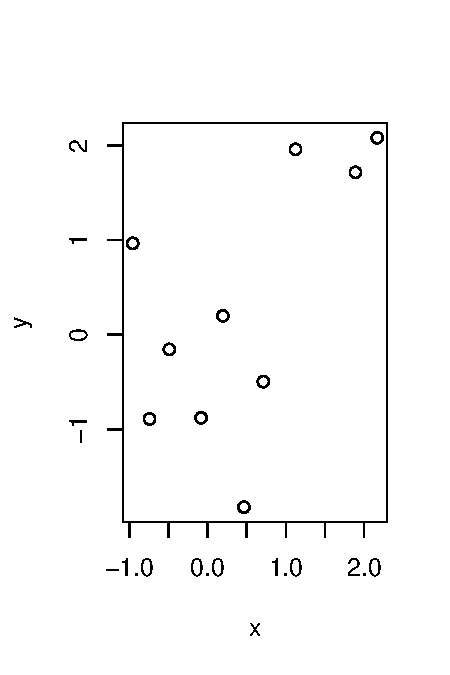
\includegraphics{ProyectoAED2023_files/figure-latex/fig1-1.pdf}
\caption{A figure added with a code chunk.\label{fig:fig1}}
\end{figure}

When making tables using \texttt{kable}, it is suggested to use the
\texttt{format="latex"} and \texttt{tabl.envir="table"} arguments to
ensure table numbering and compatibility with the mdpi document class.

\begin{table}[H]

\caption{\label{tab:tab1}This is a table caption. Tables should be placed in the 
             main text near to the first time they are~cited.}
\begin{tabular}[t]{lccc}
\toprule
  & mpg & cyl & disp\\
\midrule
Mazda RX4 & 21.0 & 6 & 160\\
Mazda RX4 Wag & 21.0 & 6 & 160\\
Datsun 710 & 22.8 & 4 & 108\\
Hornet 4 Drive & 21.4 & 6 & 258\\
Hornet Sportabout & 18.7 & 8 & 360\\
\bottomrule
\end{tabular}
\end{table}

For a very wide table, landscape layouts are allowed.

\startlandscape

\begin{table}[H]

\caption{\label{tab:tab2}This is a very wide table}
\begin{tabular}[t]{cccc}
\toprule
Title.1 & Title.2 & Title.3 & Title.4\\
\midrule
Entry 1 & Data & Data & This cell has some longer content that runs over
                               two lines\\
Entry 2 & Data & Data & Data\\
\bottomrule
\end{tabular}
\end{table}

\finishlandscape

\hypertarget{formatting-of-mathematical-components}{%
\subsection{Formatting of Mathematical
Components}\label{formatting-of-mathematical-components}}

This is an example of an equation:

\[
a = 1.
\]

If you want numbered equations use Latex and wrap in the equation
environment:

\begin{equation}
a = 1,
\end{equation}

the text following an equation need not be a new paragraph. Please
punctuate equations as regular text.

This is the example 2 of equation:

\begin{adjustwidth}{-\extralength}{0cm}
\begin{equation}
a = b + c + d + e + f + g + h + i + j + k + l + m + n + o + p + q + r + s + t + 
u + v + w + x + y + z
\end{equation}
\end{adjustwidth}

Theorem-type environments (including propositions, lemmas, corollaries
etc.) can be formatted as follows:

Example of a theorem:

\begin{Theorem}
Example text of a theorem

\end{Theorem}

The text continues here. Proofs must be formatted as follows:

Example of a proof:

\begin{proof}[Proof of Theorem1]
Text of the proof. Note that the phrase ``of Theorem 1'\,' is optional
if it is clear which theorem is being referred to.

\end{proof}

The text continues here.

\hypertarget{discussion}{%
\section{Discussion}\label{discussion}}

Authors should discuss the results and how they can be interpreted in
perspective of previous studies and of the working hypotheses. The
findings and their implications should be discussed in the broadest
context possible. Future research directions may also be highlighted.

\hypertarget{conclusion}{%
\section{Conclusion}\label{conclusion}}

This section is not mandatory, but can be added to the manuscript if the
discussion is unusually long or complex.

\hypertarget{patents}{%
\section{Patents}\label{patents}}

This section is not mandatory, but may be added if there are patents
resulting from the work reported in this manuscript.

%%%%%%%%%%%%%%%%%%%%%%%%%%%%%%%%%%%%%%%%%%

\vspace{6pt}

%%%%%%%%%%%%%%%%%%%%%%%%%%%%%%%%%%%%%%%%%%
%% optional
\supplementary{The following supporting information can be downloaded
at:\\
\linksupplementary{s1}, Figure S1: title; Table S1: title; Video S1:
title.}

% Only for the journal Methods and Protocols:
% If you wish to submit a video article, please do so with any other supplementary material.
% \supplementary{The following supporting information can be downloaded at: \linksupplementary{s1}, Figure S1: title; Table S1: title; Video S1: title. A supporting video article is available at doi: link.}

%%%%%%%%%%%%%%%%%%%%%%%%%%%%%%%%%%%%%%%%%%
\authorcontributions{For research articles with several authors, a short
paragraph specifying their individual contributions must be provided.
The following statements should be used ``X.X. and Y.Y. conceive and
designed the experiments; X.X. performed the experiments; X.X. and Y.Y.
analyzed the data; W.W. contributed reagents/materials/analysis tools;
Y.Y. wrote the paper.'\,' Authorship must be limited to those who have
contributed substantially to the work reported.}

\funding{Please add:
\texttt{This\ research\ received\ no\ external\ funding\textquotesingle{}\textquotesingle{}\ or}This
research was funded by NAME OF FUNDER grant number XXX.'\,' and and
``The APC was funded by XXX'\,'. Check carefully that the details given
are accurate and use the standard spelling of funding agency names at
\url{https://search.crossref.org/funding}, any errors may affect your
future funding.}

\institutionalreview{In this section, you should add the Institutional
Review Board Statement and approval number, if relevant to your study.
You might choose to exclude this statement if the study did not require
ethical approval. Please note that the Editorial Office might ask you
for further information. Please add ``The study was conducted in
accordance with the Declaration of Helsinki, and approved by the
Institutional Review Board (or Ethics Committee) of NAME OF INSTITUTE
(protocol code XXX and date of approval).'' for studies involving
humans. OR ``The animal study protocol was approved by the Institutional
Review Board (or Ethics Committee) of NAME OF INSTITUTE (protocol code
XXX and date of approval).'' for studies involving animals. OR ``Ethical
review and approval were waived for this study due to REASON (please
provide a detailed justification).'' OR ``Not applicable'' for studies
not involving humans or animals.}

\informedconsent{Any research article describing a study involving
humans should contain this statement. Please add
\texttt{Informed\ consent\ was\ obtained\ from\ all\ subjects\ \ involved\ in\ the\ study.\textquotesingle{}\textquotesingle{}\ OR}Patient
consent was waived due to REASON (please provide a detailed
justification).'\,' OR ``Not applicable'\,' for studies not involving
humans. You might also choose to exclude this statement if the study did
not involve humans.

Written informed consent for publication must be obtained from
participating patients who can be identified (including by the patients
themselves). Please state ``Written informed consent has been obtained
from the patient(s) to publish this paper'\,' if applicable.}

\dataavailability{We encourage all authors of articles published in MDPI
journals to share their research data. In this section, please provide
details regarding where data supporting reported results can be found,
including links to publicly archived datasets analyzed or generated
during the study. Where no new data were created, or where data is
unavailable due to privacy or ethical re-strictions, a statement is
still required. Suggested Data Availability Statements are available in
section ``MDPI Research Data Policies'' at
\url{https://www.mdpi.com/ethics}.}

\acknowledgments{All sources of funding of the study should be
disclosed. Please clearly indicate grants that you have received in
support of your research work. Clearly state if you received funds for
covering the costs to publish in open access.}

\conflictsofinterest{Declare conflicts of interest or state `The authors
declare no conflict of interest.' Authors must identify and declare any
personal circumstances or interest that may be perceived as
inappropriately influencing the representation or interpretation of
reported research results. Any role of the funding sponsors in the
design of the study; in the collection, analyses or interpretation of
data in the writing of the manuscript, or in the decision to publish the
results must be declared in this section. If there is no role, please
state `The founding sponsors had no role in the design of the study; in
the collection, analyses, or interpretation of data; in the writing of
the manuscript, an in the decision to publish the results'.}

%%%%%%%%%%%%%%%%%%%%%%%%%%%%%%%%%%%%%%%%%%
%% Optional
\sampleavailability{Samples of the compounds \ldots\ldots{} are
available from the authors.}

%% Only for journal Encyclopedia

\abbreviations{Abbreviations}{
The following abbreviations are used in this manuscript:\\

\noindent
\begin{tabular}{@{}ll}
MDPI & Multidisciplinary Digital Publishing Institute \\
DOAJ & Directory of open access journals \\
TLA & Three letter acronym \\
LD & linear dichroism \\
\end{tabular}}

%%%%%%%%%%%%%%%%%%%%%%%%%%%%%%%%%%%%%%%%%%
%% Optional
\input{"appendix.tex"}
%%%%%%%%%%%%%%%%%%%%%%%%%%%%%%%%%%%%%%%%%%
\begin{adjustwidth}{-\extralength}{0cm}

%\printendnotes[custom] % Un-comment to print a list of endnotes


\reftitle{References}
\bibliography{mybibfile.bib}

% If authors have biography, please use the format below
%\section*{Short Biography of Authors}
%\bio
%{\raisebox{-0.35cm}{\includegraphics[width=3.5cm,height=5.3cm,clip,keepaspectratio]{Definitions/author1.pdf}}}
%{\textbf{Firstname Lastname} Biography of first author}
%
%\bio
%{\raisebox{-0.35cm}{\includegraphics[width=3.5cm,height=5.3cm,clip,keepaspectratio]{Definitions/author2.jpg}}}
%{\textbf{Firstname Lastname} Biography of second author}

%%%%%%%%%%%%%%%%%%%%%%%%%%%%%%%%%%%%%%%%%%
%% for journal Sci
%\reviewreports{\\
%Reviewer 1 comments and authors’ response\\
%Reviewer 2 comments and authors’ response\\
%Reviewer 3 comments and authors’ response
%}
%%%%%%%%%%%%%%%%%%%%%%%%%%%%%%%%%%%%%%%%%%
\PublishersNote{}
\end{adjustwidth}


\end{document}
